
\section{Experimentation}
\label{sec:experimentation}

This section describes the results of our experimentation evaluating
the properties of \NAME that enables adaptive scoped broadcast in
dynamic networks. It answers the following questions: What is the
overhead of reaching consistent partitioning using \NAME in large
scale networks?  Does \NAME is relevant in Edge infrastructures where
\processes are geo-distributed into clusters? We performed the
experimentation using PeerSim, a simulator written in Java that allows
researchers to evaluate and assess distributed algorithms in large
scale networks~\cite{montresor2009peersim}. The code is available on
the Github platform at
\url{https://anonymous.4open.science/r/peersim-partition-5592}.

\subsection{Confirm the complexity analysis stating that
  communication and time overheads depend on the current partitioning
  of the system.}

\begin{asparadesc}
\item [Description:]

We build a network comprising 10k \processes. First, we chain
\processes together, then we add another communication link per
\process to another random \process. Since links are bidirectional,
each \process has 4 communication links on average. We set the latency
of links between 20 and 40 ms at random following a uniform
distribution. We set the weight of links between 5 and 15 at random
following a uniform distribution. Weights and latency are different,
hence the first $\alpha$ received by a \process may not be that of its
shortest path. It implies more concurrent operations, hence more
traffic to reach consistent partitioning.

\noindent We evaluate dynamic consistent partitioning. First, we
create 100 partitions one at a time: \processes reach consistent
partitioning before we create each new partition. Second, we remove
every partition one at a time, in the order of their creation, hence
starting from the first and oldest partition that had been added.

\noindent We focus on the complexity of \NAME. We measure the average
number of messages generated per \process per second during the
experiment; and the time before reaching consistent partitioning after
adding or removing a partition.

\item [Results:]

Figure~\ref{fig:complexity} shows the results of this experiment. The
top part shows the average traffic per \process per second divided
between $\alpha$ and $\delta$ messages. The bottom part shows the time
before reaching consistent partitioning.

\noindent Figure~\ref{fig:complexity} confirms that \NAME's overhead
depends on the size of partitions. The first partition is the most
expensive, for $\alpha$'s must reach every \process which takes time
and generate more traffic.  \NAME quickly converges towards consistent
partitioning in only 350 milliseconds. The last and $100^{th}$
partition added around 21 seconds is the least expensive. By using
scoped broadcast, control information only reaches a small subset of
the whole network.

\noindent Figure~\ref{fig:complexity} also confirms that \NAME's
delete operations are more expensive than add operations. Indeed, the
top part of the figure shows that after 21 seconds, when the
experiment involves removals, traffic includes both $\alpha$'s and
$\delta$'s. The latter aims at removing stale information and
triggering competition while the former aims at updating shortest
paths. As corollary, the convergence time increases, for $\delta$
messages must reach the partition borders before sound competitors
propagate their partition. It is worth noting that this delete
operation involves concurrency: removals continue to propagate while
the competition is already partially triggered and propagating.

\begin{figure}
  \centering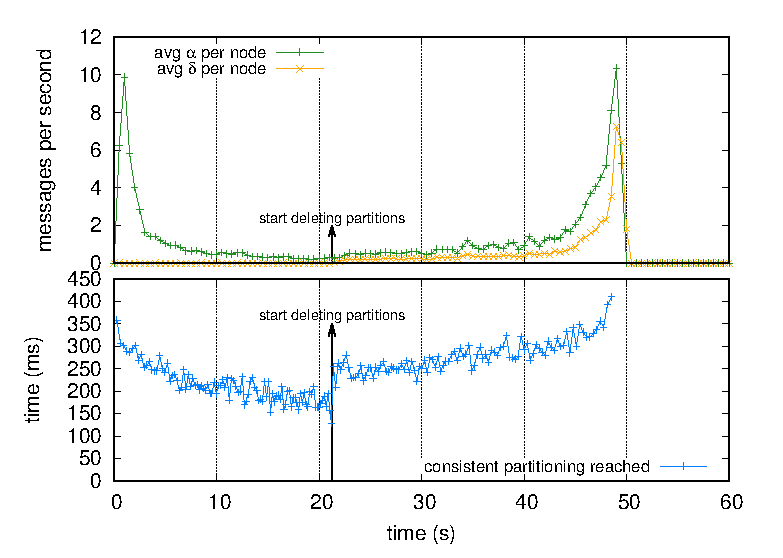
\includegraphics[width=0.99\columnwidth]{img/as_cast_complexity.eps}
  \caption{\label{fig:complexity}Overhead of consistent partitioning
    using \NAME.}
  %% \caption{\label{fig:complexity}Cumulative average number of messages
  %%   per process in a network comprising 10k processes; along with the
  %%   duration before reaching consistent partitioning after adding or
  %%   removing a partition, totaling 100 new partition then removed.}
\end{figure}

\noindent Figure~\ref{fig:complexity} shows that the overhead of
adding the $1^{st}$ partition does not correspond to the overhead of
deleting this $1^{st}$ partition. When adding it, messages must reach
all \processes while when removing it, messages must reach a small
subset of this membership.  \NAME's overhead actually depends on
current partitioning as opposed to past partitionings.

\noindent Finally, Figure~\ref{fig:complexity} highlights that after
49 seconds, i.e., after the 100 adds and the 100 deletes, \processes
do not generate traffic anymore. Being reactive, \NAME has no overhead
when there is no operation in the system. In other words, \NAME's
overhead actually depends on its usage.

\end{asparadesc}

%% \subsection{Distribution and hotspots}

% \subsection{Confirm the relevance of \NAME in the context of dynamic inter-autonomous
%   system communications.}
\subsection{Confirm that \NAME locks down the traffic of decentralized content
  indexing in the context of dynamic inter-autonomous system
  communications.}

\begin{asparadesc}
\item [Description:]

We build a network by duplicating the G{\'E}ANT
topology~\cite{knight2011internet} -- a real infrastructure spanning
across Europe -- and by connecting these two clusters with a high
latency link: $200$ ms simulating cross-continental communications
such as Europe-America. The experiments comprise $2 \times 271 = 542$
\processes and we derive intra-cluster latency from their \processes'
geographic location.

\noindent We evaluate the traffic of \NAME by measuring the average
number of messages per \process over the experiments. In the first
experiment, at $50$~ms, only one \process becomes source, hence there
is only one partition for the whole distributed system. In the second
experiment, at $50$~ms, two \processes become sources, one per
cluster. Afterwards both scenarios are identical. At $850$~ms, we
remove the link between the two clusters. At $1.7$~s, we insert back this
link.

\begin{figure}
  \centering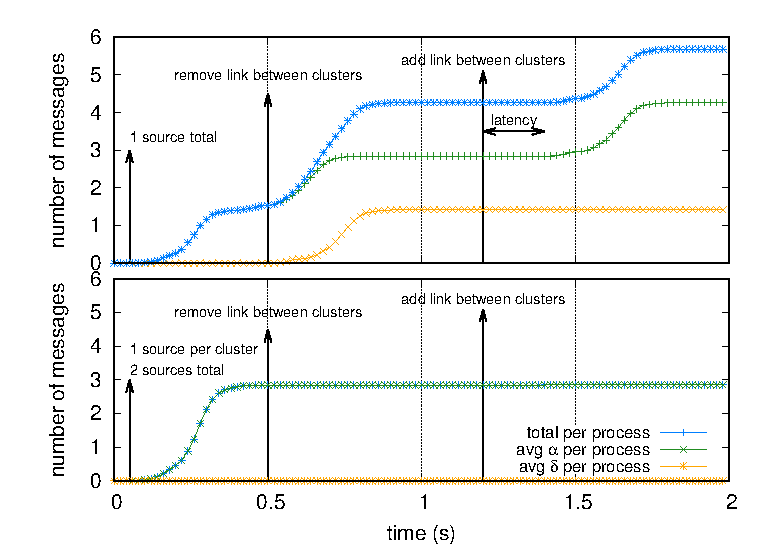
\includegraphics[width=0.99\columnwidth]{img/as_cast_geant.eps}
  \caption{\label{fig:geant}Overhead of \NAME in the partitioning of 2 clusters.}
\end{figure}

\item [Results:]

Figure~\ref{fig:geant} shows the results of this experimentation. The
top part displays the one source experiment while the bottom part
displays the one source per cluster experiment.

\noindent Figure~\ref{fig:geant} confirms that concurrent
\texttt{Add}s may reach consistent partitioning faster. In particular,
the top part of Figure~\ref{fig:geant} depicts a slow down in traffic
around $500$ ms due to the high latency inter-continental link. The
first plateau corresponds to the source's autonomous system
acknowledging this source, while the second plateau corresponds to the
other autonomous system catching up.  The inter-continental link acts
as a bottleneck that does not exist when each cluster has its own
source.

\noindent Figure~\ref{fig:geant} highlights that removing the
inter-continental link generates additional traffic. The cluster cut
off from the source must purge all control information about this
source.  Most importantly, Figure~\ref{fig:geant} shows that \NAME
still operates well when \emph{physical} partitions appear. \Processes
from the cluster without source do not belong to any partition while
\processes from the other cluster belong to the same partition. 

\noindent Figure~\ref{fig:geant} shows that, when adding back the
inter-continental link, the two clusters can communicate again. In the
experiment involving one source for two clusters, it generates
traffic. After a $200$ milliseconds delay corresponding to the link latency, the
cut off cluster starts to communicate $\alpha$ messages
again. Eventually, all \processes belong to the same
partition. However, in the experiment involving one source \emph{per}
cluster, the new link does not trigger noticeable traffic, for
\processes already know their closest source located in their
respective cluster.

\noindent Overall, this experimentation empirically demonstrates the
benefits of \NAME in the context of geo-distributed infrastructures,
e.g., inter-connected autonomous systems where \processes and
communications links may be added and removed at any time. \NAME
coupled with replication strategies designed for Edge infrastructures
would allow locking down the traffic of replica indexing, while
providing every \process with quick access to replicated content.

\end{asparadesc}

Next Section reviews state-of-the-art approaches for content indexing
in geo-distributed infrastructures and explains their shortcomings.

% \subsection{Use case: caching}
% \subsection{Use case: routing}
% \subsection{Use case: broadcast domain}


%%% Local Variables: 
%%% mode: latex
%%% TeX-master: "../paper"
%%% ispell-local-dictionary: "english"
%%% End: 
